\chapter{Network models}
\label{Network-models}

Throughout this chapter, we discuss the specification of \texttt{Network} models. %Instead, we point to the following chapters for \texttt{CacheNetwork} and \texttt{LayeredNetwork} models.
It is important to keep in mind that not all of the model features described in the present chapter are supported by every
\textsc{Line} solver. However, upon calling a solver, \textsc{Line} will automatically detect if the supplied model can be
analyzed by that solver and return an empty set if not. Tables are given later in the manual summarizing the features supported by each solver.

\section{Network object definition}
\label{network-object-definition}
\subsection{Creating a network and its nodes}
A queueing network can be described in \textsc{Line} using the \texttt{Network} class constructor with a unique string identifying the model name:
\begin{lstlisting}
model = Network('myModel');
\end{lstlisting}
The returned object of the \texttt{Network} class offers functions to instantiate and manage resource \emph{nodes} (stations,  delays, caches, ...) visited by jobs of several types (\emph{classes}).

A {node} is a resource in the network that can be visited by a job. A node must have a unique name and can either be {\em stateful} or {\em stateless}, the latter meaning that the node does not require state variables to determine the actions it performs on the system. If jobs visiting a stateful node can be required to spend time in it, the node is also said to be a {\em station}. A list of nodes available in \texttt{Network} models is given in the next table.

\begin{table}[h!]
\caption{Nodes available in \texttt{Network} models.}
\begin{tabular}{|l|l|p{9.7cm}|}
\hline
{Node} & {Type} & {Description} \\
\hline
\texttt{Cache} & stateful node & A class-switching router based on cache hits/misses\\
\texttt{ClassSwitch} & stateless node & A class-switching router based on a static probability matrix\\
\texttt{Delay} & station & A station where jobs spend time without queueing\\
%\texttt{Logger} & stateless node & A node that logs passage of jobs\\
\texttt{Queue} & station & A generic queueing element\\
%\texttt{Router} & stateful node & A node that routes jobs\\
\texttt{Sink} & stateless node & Exit point for jobs in open classes\\
\texttt{Source} & station & Entry point for jobs in open classes\\
\hline
\end{tabular}
\end{table}

For example, a sink is a stateless node, since its behaviour does not require state variables and jobs cannot sojourn in it. Instead, a first-come first-served queue is a station, since jobs can sojourn inside its buffer and servers. A source is also treated in \textsc{Line} as a station since the inter-arrival time of jobs from the external world is considered as a time spent in the source, although this is not counted as part of the system response time.
Lastly, a cache is a stateful node, since it needs to keep track of the cached items, however it is not a station since passage through this node occurs instantaneously.

We now provide more details on each of the nodes available in \texttt{Network} models.
\paragraph{Queue node.}
Among the listed nodes, the most important one is the \texttt{Queue}, which specifies a queueing station from its name and scheduling strategy, e.g.
\begin{lstlisting}
queue = Queue(model, 'Queue1', SchedStrategy.FCFS);
\end{lstlisting}
It is also possible to instantiate a queue using the \texttt{QueueingStation} constructor, which is merely an alias for the \texttt{Queue} class.

Valid scheduling strategies are specified within the \texttt{SchedStrategy} static class and include:
\begin{itemize}
\item First-come first-served (\texttt{SchedStrategy.FCFS})
\item Infinite-server (\texttt{SchedStrategy.INF})
\item Processor-sharing (\texttt{SchedStrategy.PS})
\item Discriminatory processor-sharing (\texttt{SchedStrategy.DPS})
\item Generalized processor-sharing (\texttt{SchedStrategy.GPS})
\item Shortest expected processing time (\texttt{SchedStrategy.SEPT})
\item Shortest job first (\texttt{SchedStrategy.SJF})
\item Head-of-line priority (\texttt{SchedStrategy.HOL})
\end{itemize}
If a strategy requires class weights, these can be specified directly as an argument to the \texttt{setService} function or using the \texttt{setStrategyParam} function, see later the description of DPS scheduling for an example.

\paragraph{Delay node.} Infinite-server stations may be instantiated either as objects of \texttt{Queue} class with the \texttt{SchedStrategy.INF} strategy or using the following specialized constructor
\begin{lstlisting}
delay = Delay(model, 'ThinkTime');
\end{lstlisting}
As for queues, for readability it is possible to instantiate delay nodes using the \texttt{DelayStation} constructor, which is entirely equivalent to the one of the \texttt{Delay} class.

\paragraph{Source and Sink nodes.} As seen in the M/M/1 getting started example, these nodes are mandatory elements for the specification of open classes. Their constructor only requires a specification of the unique name associated to the nodes:
\begin{lstlisting}
source = Source(model, 'Source');
sink = Sink(model, 'Sink');
\end{lstlisting}

\paragraph{ClassSwitch node.} This is a stateless node to change the class of a transiting job based on a static probabilistic policy. For example, it is possible to specify that all jobs belonging to class 1 should become of class 2, or that a class 2 job should become of class 1 with probability $0.3$. This example is instantiated as follows
\begin{lstlisting}
cs = ClassSwitch(model, 'ClassSwitchPoint',[0.0, 1.0; 0.3, 0.7]);
\end{lstlisting}

\paragraph{Cache node.} This is a stateful node to store one or more items in a cache of finite size, for which it is possible to specify a replacement policy.  The cache constructor requires the total cache capacity and the number of items that can be referenced by the jobs in transit, e.g.,
\begin{lstlisting}
cacheNode = Cache(model, 'Cache1', nitems, capacity, ReplacementPolicy.LRU);
\end{lstlisting}
If the capacity is an integer (e.g., \texttt{[15]}) , then it represents the total number of items that can be cached and the value cannot be greater than the number of items. Conversely, if it is a vector (e.g., \texttt{[10,5]}) then the node is a list-based cache, where the vector entries specify the capacity of each list. We point to \cite{GastH16} for more details on list-based caches and their replacement policies.

Available replacement policies are specified within the \texttt{ReplacementPolicy} static class and include:
\begin{itemize}
\item First-in first-out (\texttt{ReplacementPolicy.FIFO})
\item Random replacement (\texttt{ReplacementPolicy.RAND})
\item Least-recently used (\texttt{ReplacementPolicy.LRU})
\item Strict first-in first-out (\texttt{ReplacementPolicy.SFIFO})
\end{itemize}
Upon cache hit or cache miss, a job in transit is switched to a user-specified class. More details are given later in Section~\ref{class-switching}.

\subsection{Job classes}
Jobs travel within the network placing service demands at the stations. The demand placed by a job at a station depends on the class of the job. Jobs in {\em open classes} arrive from the external world and, upon completing the visit, leave the network. Jobs in {\em closed classes} start within the network and are forbidden to ever leave it, perpetually cycling among the nodes.

\subsubsection{Open classes}
The constructor for an open class only requires the class name and the creation of special nodes called \texttt{Source} and \texttt{Sink}
\begin{lstlisting}
source = Source(model, 'Source');
sink = Sink(model, 'Sink');
\end{lstlisting}
Sources are special stations holding an infinite pool of jobs and representing the external world. Sinks are nodes that route a departing job back into this infinite pool, i.e., into the source. Note that a network can include at most a single \texttt{Source} and a single \texttt{Sink}.

Once source and sink are instantiated in the model, it is possible to instantiate open classes using
\begin{lstlisting}
class1 = OpenClass(model, 'Class1');
\end{lstlisting}
\textsc{Line} does not require to associate source and sink with the open classes in their constructors, as this is done automatically. However, the \textsc{Line} language requires to explicitly create these nodes since the routing topology needs to indicate the arrival and departure points of jobs in open classes. However, if the network does not includes open classes, the user will not need to instantiate a \texttt{Source} and a \texttt{Sink}.

\subsubsection{Closed classes}
To create a closed class, we need instead to indicate the number of jobs that start in that class (e.g., 5 jobs) and the {\em reference station} for that class (e.g., \texttt{queue}), i.e.:
\begin{lstlisting}
class2 = ClosedClass(model, 'Class2', 5, queue);
\end{lstlisting}
The reference station indicates a point in the network used to calculate certain performance indexes, called {\em system performance indexes}. The end-to-end response time for a job in an open class to traverse the system is an example of system performance index (system response time). The reference station of an open class is always automatically set by \textsc{Line} to be the \texttt{Source}. Conversely the reference station needs to be indicated explicitly in the constructor for closed classes, since the point at which a class job completes execution depends on the semantics of the model.

\subsubsection{Mixed models}
\textsc{Line} also accepts models where a user has instantiated both open and closed classes. The only requirement is that, if two classes communicate by means of a class-switching mechanism, then the two classes must either be all closed or all open. In other words, classes in the same chain must either be both closed or both open. Furthermore, for closed classes in the same chain it is required that the reference station is the same.

\subsubsection{Class priorities}
If a class has a priority, with 0 representing the highest priority, this can be specified as an additional argument to both \texttt{OpenClass} and \texttt{ClosedClass}, e.g.,
\begin{lstlisting}
class2 = ClosedClass(model, 'Class2', 5, queue, 0);
\end{lstlisting}
In \texttt{Network} models, priorities are intended as hard priorities and the only supported priority scheduling strategy (\texttt{SchedStrategy.HOL}) is non-preemptive. Weight-based policies such as DPS and GPS may be used, as an alternative, to prevent starvation of jobs in low priority classes.

\subsection{Routing strategies}
\subsubsection{Probabilistic routing}
Jobs travel between nodes according to the network topology and a routing strategy. Typically a queueing network will use a probabilistic routing strategy (\texttt{RoutingStrategy.PROB}), which requires to specify routing probabilities among the nodes. The simplest way to specify a large routing topology is to define the routing probability matrix for each class, followed by a call to the \texttt{link} function. This function will automatically add certain nodes to the network to ensure the correct switching of class for jobs moving between stations (\texttt{ClassSwitch} elements).

In the running case, we may instantiate a routing topology as follows:
\begin{lstlisting}
P = cellzeros(2,4);
P{class1}(source,queue) = 1.0;
P{class1}(queue,[queue,delay]) = [0.3,0.7]; % self-loop with probability 0.3
P{class1}(delay,sink) = 1.0;
P{class2}(delay,queue) = 1.0; % closed class starts at delay
P{class2}(queue,delay) = 1.0;
model.link(P);
\end{lstlisting}
When used as arguments to a cell array or matrix, class and node objects will be replaced by a corresponding numerical index.
Normally, the indexing of classes and nodes matches the order in which they are instantiated in the model and one can therefore specify the routing matrices using this property. In this case we would have
\begin{lstlisting}
P = cellzeros(2,4);
P{class1} = [0,1,0,0;   % row: source
             0,.3,.7,0; % row: queue
             0,0,0,1;   % row: delay
             0,0,0,0];  % row: sink
P{class2} = [0,0,0,0;
             0,0,1,0;
             0,1,0,0;
             0,0,0,0];
model.link(P);
\end{lstlisting}
The \texttt{getClassIndex} and \texttt{getNodeIndex} functions return the numerical index associated to a node name, e.g.,
\texttt{model.getNodeIndex('Delay')}. Class and node names in a network need to be unique. The list of used names can be obtained with the \texttt{getClassNames}, \texttt{getStationNames}, and \texttt{getNodeNames} functions of the \texttt{Network} class.

It is also important to note that the routing matrix in the last example is specified between {\em nodes}, instead than between just stations or stateful nodes, which means that elements such as the \texttt{Sink} need to be explicitly considered in the routing matrix. The only exception is that \texttt{ClassSwitch} elements do not need to be explicitly instantiated and explicited in the routing matrix, provided that one uses the \texttt{link} function to instantiate the topology. Note that the routing matrix assigned to a model can be printed on screen in human-readable format using the \texttt{printRoutingMatrix} function.

\subsubsection{Other routing strategies}
The above routing specification style is only for models with probabilistic routing strategies between every pair of nodes. A different style should be used for scheduling policies that do not require to explicit routing probabilities, as in the case of state-dependent routing. Currently supported strategies include:
\begin{itemize}
\item Round robin (\texttt{RoutingStrategy.RR}). This is a non-probabilistic strategy that sends jobs to outgoing links in a cyclic order. %It is currently supported only by \texttt{SolverJMT}.
\item Random routing (\texttt{RoutingStrategy.RAND}). This is equivalent to a standard probabilistic strategy that for each class assigns identical values to the routing probabilities of all outgoing links.
\item Join-the-Shortest-Queue (\texttt{RoutingStrategy.JSQ}).  This is a non-probabilistic strategy that sends jobs to the destination with the smallest total number of jobs in it. If multiple stations have the same total number of jobs, then the destination is chosen at random with equal probability across these stations.
\end{itemize}
For such policies, the function \texttt{addLink} should be first used to specify pairs of connected nodes
\begin{lstlisting}
model.addLink(queue, queue); %self-loop
model.addLink(queue, delay);
\end{lstlisting}
Then an appropriate routing strategy should be selected at every node, e.g.,
\begin{lstlisting}
queue.setRouting(class1,RoutingStrategy.RR);
\end{lstlisting}
assigns round robin among all outgoing links from the \texttt{queue} node.

A model could also include both classes with probabilistic routing strategies and classes that use round robin or other non-probabilistic startegies. To instantiate routing probabilities in such situations one should then use, e.g.,
\begin{lstlisting}
queue.setRouting(class1,RoutingStrategy.PROB);
queue.setProbRouting(class1, queue, 0.7)
queue.setProbRouting(class1, delay, 0.3)
\end{lstlisting}
where \texttt{setProbRouting} assigns the routing probabilities to the two links.

\subsection{Class switching}
\label{class-switching}

In \textsc{Line}, jobs can switch class while they travel between nodes (including self-loops on the same node). For example, this feature can be used to model queueing properties such as re-entrant lines in which a job visiting a station a second time may require a different average service demand than at its first visit.

A chain defines the set of reachable classes for a job that starts in the given class $r$ and over time changes class. Since class switching in \textsc{Line} does not allow a closed class to become open, and vice-versa, chains can themselves be classified into {\em open chains} and {\em closed chains}, depending on the classes that compose them.

Jobs in open classes can only switch to another open class. Similarly, jobs in closed classes can only switch to a closed class. Thus, class switching from open to closed classes (or vice-versa) is forbidden. The strategy to describe the class switching mechanism is integrated in the specification of the routing between stations as described next.

\subsubsection{Probabilistic class switching}
In models with class switching and probabilistic routing at all nodes, a routing matrix is required for each possible pair of source and target classes. For example, suppose that in the previous example the job in the closed class \texttt{class2} switches into a new closed class (\texttt{class3}) while visiting the \texttt{queue} node. We can specify this routing strategy as follows:
\begin{lstlisting}
class3 = ClosedClass(model, 'Class3', 0, queue, 0);

P = cellzeros(3,3,4);
P{class1,class1}(source, queue) = 1.0;
P{class1,class1}(queue, [queue,delay]) = [0.3,0.7];
P{class1,class1}(delay, sink) = 1.0;
P{class2,class3}(delay, queue) = 1.0; % closed class starts at delay
P{class3,class2}(queue, delay) = 1.0;
model.link(P);
\end{lstlisting}
where \texttt{P\{r,s\}} is the routing matrix for jobs switching from class \texttt{r} to \texttt{s}. That is, \texttt{P\{r,s\}(i,j)} is the probability that a job in class \texttt{r} departs node \texttt{i} routing into node \texttt{j} as a job of class \texttt{s}.

Importantly, \textsc{Line} assumes that a job switches class an instant {\em after} leaving a station, thus the performance metrics of a class at the node refer to the class that jobs had upon arrival to that node.

Depending on the specified probabilities, a job will be able to switch class only among a subset of the available classes. Each subset is called a {\em chain}. Chains are computed in \textsc{Line} as the weakly connected components of the routing probability matrix of the network, when this is seen as an undirected graph. The function \texttt{model.getChains} produces the list of chains for the model, inclusive of a list of their composing classes.

An advanced feature of \textsc{Line} available for example within the \texttt{Cache} node, is that the class-switching decision can dynamically depend on the state of the node (e.g., cache hit/cache miss). However, in order to statically determine chains, \textsc{Line} requires that every class-switching node declares the pair of classes that can potentially communicate with each other via a switch. This is called the {\em class-switching mask} and it is automatically computed. The boolean matrix returned by the \texttt{model.getClassSwitchingMask} function provides this mask, which has entry in row $r$ and column $s$ set to true only if jobs in class $r$ can switch into class $s$ at some node in the network.

\subsubsection{Class switching with non-probabilistic routing strategies}
In the presence of non-probabilistic routing strategies, one needs to specify more details of the class switching mechanism. This can be done through addition to the network topology of \texttt{ClassSwitch} elements. The constructor of this node requires to specify a probability matrix $C$ such that $C(r,s)$ is the probability that a job of class $r$ arriving into the \texttt{ClassSwitch} switches to class $s$ during the visit. For example, in a 2-class model the following node will switch all visiting jobs into class 2
\begin{lstlisting}
C = [0, 1; 0, 1];
node = ClassSwitch(model, 'CSNode',C);
\end{lstlisting}
Note that for a network with $M$ stations, up to $M^2$ \texttt{ClassSwitch} elements may be required to implement class-switching across all possible links, including self-loops. Moreover, refreshing network parameters under non-probabilistic routing strategies may .

Contrary to the \texttt{link} function, one cannot specify in the argument to \texttt{setProbRouting} a class switching probability. The \texttt{setProbRouting} function should instead be used to route the job through an appropriate \texttt{ClassSwitch} element.

\subsubsection{Routing probabilities for Source and Sink nodes}
In the presence of open classes, and in mixed models with both open and closed classes, one needs only to specify the routing probabilities {\em out} of the source. The probabilities out of the sink can all be set to zero for all classes and destinations (including self-loops). The solver will take care of adjusting these inputs to create a valid routing table.

\subsubsection{Cache-based class-switching}
\label{cache-based-class-switching}
Upon cache hit or cache miss, a job in transit is switched to a user-specified class, as specified by the \texttt{setHitClass} and \texttt{setMissClass}, so that it can be routed to a different destination based on wether it found the item in the cache or not. The \texttt{setRead} function allows the user to specify a discrete distribution (e.g., \texttt{Zipf}, \texttt{DiscreteDistrib}) for the frequency at which an item is requested. For example,
\begin{lstlisting}
refModel = Zipf(0.5,nitems);
cacheNode.setRead(initClass, refModel);
cacheNode.setHitClass(initClass, hitClass);
cacheNode.setMissClass(initClass, missClass);
\end{lstlisting}
Here \texttt{initClass}, \texttt{hitClass}, and \texttt{missClass} can be either open or closed instantiated as usual with the \texttt{OpenClass} or \texttt{ClosedClass} constructors.

\subsubsection{Reference station}
\label{reference-station}
Before we have shown that the specification of classes requires to choose a reference station. In \textsc{Line}, reference stations are properties of chains, thus if two closed classes belong to the same chain they must have the same reference station. This avoids ambiguities in the definition of the completion point for jobs within a chain.

For example, the system throughput for a chain is defined as sum of the arrival rates at the reference station for all classes in that chain. That is, the solver counts a return to the reference station as a completion of the visit to the system. In the case of open chains, the reference station is always the \texttt{Source} and the system throuhput corresponds to the rate at which jobs arrive to the sink \texttt{Sink}, which may be seen as the arrival rate seen by the infinite pool of jobs in the external world. If there is no class switching, each chain contain a single class, thus per-chain and per-class performance indexes will be identical.


\subsubsection{Tandem and cyclic topologies}
Tandem networks are open queueing networks with a serial topology. \textsc{Line} provides functions that ease the definition of tandem networks of stations with exponential service times. For example, we can rapidly instantiate a tandem network consisting of stations with PS and INF scheduling as follows
\begin{lstlisting}
A = [10,20]; % A(r) - arrival rate of class r
D = [11,12; 21,22]; % D(i,r) - class-r demand at station i (PS)
Z = [91,92; 93,94]; % Z(i,r)  - class-r demand at station i (INF)
modelPsInf = Network.tandemPsInf(A,D,Z)
\end{lstlisting}
The above snippet instantiates an open network with two queueing stations (PS), two delay stations (INF), and exponential distributions with the given inter-arrival rates and mean service times. The \texttt{Network.tandemPs}, \texttt{Network.tandemFcfs}, and \texttt{Network.tandemFcfsInf} functions provide static constructors for networks with other combinations of scheduling policies, namely only PS, only FCFS, or FCFS and INF.

A tandem network with closed classes is instead called a cyclic network. Similar to tandem networks, \textsc{Line} offers a set of static constructors: \texttt{Network.cyclicPs}, \texttt{Network.cyclicPsInf}, \texttt{Network.cyclicFcfs}, and \texttt{Network.cyclicFcfsInf}. These functions only require to replace the arrival rate vector \texttt{A} by a vector \texttt{N} specifying the job populations for each of the closed classes, e.g.,
\begin{lstlisting}
N = [10,20]; % N(r) - closed population in class r
D = [11,12; 21,22]; % D(i,r) - class-r demand at station i (PS)
modelPsInf = Network.cyclicPs(N,D)
\end{lstlisting}

\subsection{Finite buffers}
The functions \texttt{setCapacity} and \texttt{setChainCapacity} of the \texttt{Station} class are used to place constraints on the number of jobs, total or for each chain, that can reside within a station. Note that \textsc{Line} does not allow one to specify buffer constraints at the level of individual classes, unless chains contain a single class, in which case \texttt{setChainCapacity} is sufficient for the purpose.

For example,
\begin{lstlisting}
example_closedModel_3
delay.setChainCapacity([1,1])
model.refreshCapacity()
\end{lstlisting}
creates an example model with two chains and three classes (specified in \texttt{example\_closedModel\_3.m}) and requires the second station to accept a maximum of one job in each chain. Note that if we were to ask for a higher capacity, such as \texttt{setChainCapacity([1,7])}, which exceeds the total job population in chain 2, \textsc{Line} would have automatically reduced the value 7 to the chain 2 job population (2). This automatic correction ensures that functions that analyze the state space of the model do not generate unreachable states.

The \texttt{refreshCapacity} function updates the buffer parameterizations, performing appropriate sanity checks. Since \texttt{example\_closedModel\_3} has already invoked a solver prior to our changes, the requested modifications are materially applied by \textsc{Line} to the network only after calling an appropriate \texttt{refreshStruct} function, see the sensitivity analysis section. If the buffer capacity changes were made before the first solver invocation on the model, then there would not be need for a \texttt{refreshCapacity} call, since the internal representation of the \texttt{Network} object used by the solvers is still to be created.

\subsection{Service and inter-arrival time processes}
\label{service-and-inter-arrival-time-processes}
A number of statistical distributions are available to specify job service times at the stations and inter-arrival times from the \texttt{Source} station. The class \texttt{PhaseType} offers distributions that are analytically tractable, which are defined upon certain absorbing Markov chains consisting of one or more states ({\em phases}) that are called phase-type distributions. They include as special case the following distributions supported in \textsc{Line}, along with their respective constructors:
\begin{itemize}
\item Exponential distribution: \texttt{Exp}$(\lambda)$, where $\lambda$ is the rate of the exponential
\item $n$-phase Erlang distribution: \texttt{Erlang}$(\alpha, n)$, where $\alpha$ is the rate of each of the $n$ exponential phases
\item $2$-phase hyper-exponential distribution: \texttt{HyperExp}$(p,\lambda_1,\lambda_2)$, that returns an exponential with rate $\lambda_1$ with probability $p$, and  an exponential with rate $\lambda_2$ otherwise.
\item $2$-phase Coxian distribution: \texttt{Cox2}$(\mu_1,\mu_2,\phi_1)$, which assigns rates $\mu_1$ and $\mu_2$ to the two rates, and completion probability from phase 1 equal to $\phi_1$ (the probability from phase 2 is $\phi_2=1.0$).
\end{itemize}
For example, given mean $\mu=0.2$ and squared coefficient of variation SCV=10, where SCV=variance/$\mu^2$, we can assign to a node a $2$-phase Coxian service time distribution with these moments as
\begin{lstlisting}
queue.setService(class2, Cox2.fitMeanAndSCV(0.2,10));
\end{lstlisting}
Inter-arrival time distributions can be instantiated in a similar way, using \texttt{setArrival} instead of \texttt{setService} on the \texttt{Source} node. For example, if the \texttt{Source} is node 3 we may assign the inter-arrival times of class 2 to be exponential with mean 0.1 as follows
\begin{lstlisting}
source.setArrival(class2, Exp.fitMeanAndSCV(0.1));
\end{lstlisting}
where we have used a single parameter in \texttt{fitMeanAndSCV} since the exponential distribution does not allow to choose the SCV.

Non-Markovian distributions are also available, but typically they restrict the available network analysis techniques to simulation. They include the following distributions:
\begin{itemize}
\item Deterministic distribution: \texttt{Det}$(\mu)$ assigns probability 1.0 to the value $\mu$.
\item Uniform distribution: \texttt{Uniform}$(a,b)$ assigns uniform probability $1/(b-a)$ to the interval $[a,b]$.
\item Gamma distribution: \texttt{Gamma}$(\alpha, k)$ assigns a gamma density with shape $\alpha$ and scale $k$.
\item Pareto distribution: \texttt{Pareto}$(\alpha, k)$ assigns a Pareto density with shape $\alpha$ and scale $k$.
\end{itemize}

Lastly, we discuss two special distributions. The \texttt{Disabled} distribution can be used to explicitly forbid a class to receive service at a station. This may be useful in models with sparse routing matrices, both to ensure an efficient model solution and to debug the model specification. Performance metrics for disabled classes will be set to \texttt{NaN}.

Conversely, the \texttt{Immediate} class can be used to specify instantaneous service (zero service time). Typically, \textsc{Line} solvers will replace zero service times with small positive values ($\varepsilon=10^{-7}$).

\subsubsection{Fitting a distribution}
The \texttt{fitMeanAndSCV} function is available for all distributions that inherit from the \texttt{PhaseType} class. This function provides exact or approximate matching of the requested moments, depending on the theoretical constraints imposed by the distribution. For example, an Erlang distribution with SCV=0.75 does not exist, because in a $n$-phase Erlang it must be SCV=$1/n$. In a case like this, \texttt{Erlang.fitMeanAndSCV(1,0.75)} will return the closest approximation, e.g., a 2-phase Erlang (SCV=0.5) with unit mean. The Erlang distribution also offer a function \texttt{fitMeanAndOrder}$(\mu,n)$, which instantiates a $n$-phase Erlang with given mean $\mu$.

In distributions that are uniquely determined by more than two moments, \texttt{fitMeanAndSCV} chooses a particular assignment of the residual degrees of freedom other than mean and SCV. For example, \texttt{HyperExp} depends on three parameters, therefore it is insufficient to specify mean and SCV to identify the distribution. Thus, \texttt{HyperExp.fitMeanAndSCV} automatically chooses to return a probability of selecting phase 1 equal to 0.99, as this spends the degree of freedom corresponding to the (unspecified) third moment of the distribution. Compared to other choices, this particular assignment corresponds to an higher probability mass in the tail of the distribution.

\subsubsection{Inspecting and sampling a distribution}
To verify that the fitted distribution has the expected mean and SCV it is possible to use the \texttt{getMean} and \texttt{getSCV} functions, e.g.,
\begin{lstlisting}
>> dist = Exp(1);
>> dist.getMean
ans =
     1
>> dist.getSCV
ans =
     1
\end{lstlisting}
Moreover, the \texttt{sample} function can be used to generate values from the obtained distribution, e.g. we can generate 3 samples as
\begin{lstlisting}
>> dist.sample(3)
ans =
    0.2049
    0.0989
    2.0637
\end{lstlisting}
The \texttt{evalCDF} and \texttt{evalCDFInterval} functions return the cumulative distribution function at the specified point or within a range, e.g.,
\begin{lstlisting}
>> dist.evalCDFInterval(2,5)
ans =
    0.1286
>> dist.evalCDF(5)-dist.evalCDF(2)
ans =
    0.1286
\end{lstlisting}
For more advanced uses, the distributions of the \texttt{PhaseType} class also offer the possibility to obtain the standard $(D_0,D_1)$ representation used in the theory of Markovian arrival processes by means of the \texttt{getRenewalProcess} function. The result will be a cell array where element $k+1$ corresponds to matrix $D_k$.

\subsubsection{Temporal dependent processes}
It is sometimes useful to specify the statistical properties of a {\em time series} of service or inter-arrival times, as in the case of systems with short- and long-range dependent workloads. When the model is stochastic, we refer to these as situations where one specifies a {\em process}, as opposed to only specifying the {\em distribution} of the service or inter-arrival times. In \textsc{Line} processes inherit from the \texttt{PointProcess} class, and include the 2-state Markov-modulated Poisson process (\texttt{MMPP2}) and empirical traces read from files (\texttt{Replayer}).

In particular, \textsc{Line} assumes that empirical traces are supplied as text files (ASCII), formatted as a column of numbers. Once specified, the \texttt{Replayer} object can be used as any other distribution. This means that it is possible to run a simulation of the model with the specified trace. However, analytical solvers will require tractable distributions from the \texttt{PhaseType} class.

\subsubsection{Scheduling parameters}
\label{scheduling-parameters}
Upon setting service distributions at a station, one may also specify scheduling parameters such as weights as additional arguments to the \texttt{setService} function. For example, if the node implements discriminatory processor sharing (\texttt{SchedStrategy.DPS}), the command
\begin{lstlisting}
queue.setService(class2, Cox2.fitMeanAndSCV(0.2,10), 5.0);
\end{lstlisting}
assigns a weight 5.0 to jobs in class 2. The default weight of a class is 1.0.

\subsection{Debugging and visualization}
JSIMgraph is the graphical simulation environment of the JMT suite. \textsc{Line} can export models to this environment for visualization purposes using the command
\begin{lstlisting}
model.jsimgView
\end{lstlisting}
An example is shown in Figure~\autoref{jsimgView-function} below. Using a related function, \texttt{jsimwView}, it is also possible to export the model to the JSIMwiz environment, which offers a wizard-based interface.
\begin{figure}
  \centering
  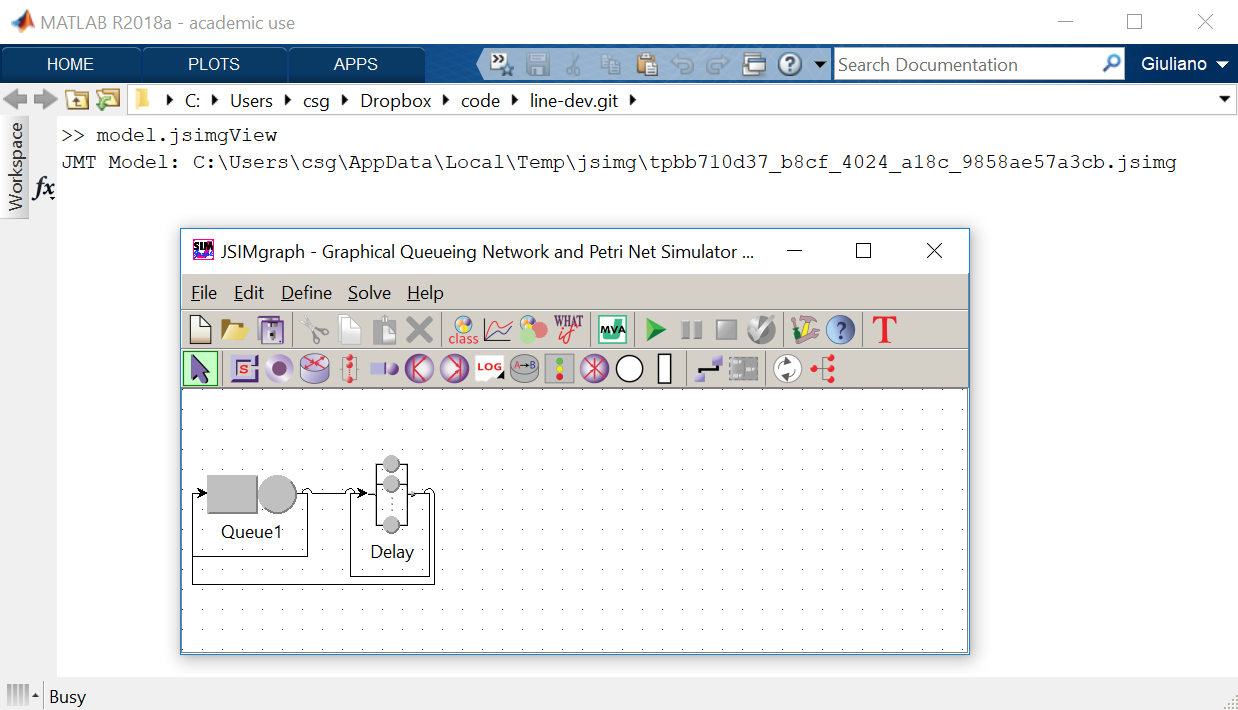
\includegraphics[width=14cm]{./images/jsimgView.png}
%  \caption{\texttt{Network.jsimgView} function}\label{FIG_jsimgView}
  \caption{jsimgView function}\label{jsimgView-function}
\end{figure}

Another way to debug a \textsc{Line} model is to transforming it into a MATLAB graph object, e.g.
\begin{lstlisting}
G = model.getGraph();
plot(G,'EdgeLabel',G.Edges.Weight,'Layout','Layered')
\end{lstlisting}
plots a graph of the network topology in term of stations only. In a similar manner, the following variant of the same command shows the model in terms of nodes, which corresponds to the internal representation within \textsc{Line}.
\begin{lstlisting}
[~,H] = model.getGraph();
plot(H,'EdgeLabel',H.Edges.Weight,'Layout','Layered')
\end{lstlisting}
The next figures shows the difference between the two commands for an open queueing network with two classes and class-switching. Weights on the edges correspond to routing probabilities. In the station topology on the left, note that since the \texttt{Sink} node is not a station, departures to the \texttt{Sink} are drawn as returns to the \texttt{Source}. The node topology on the right, illustrates all nodes, including certain \texttt{ClassSwitch} nodes that are automatically added by \textsc{Line} to apply the class-switching routing strategy. Double arcs between nodes indicate that both classes are routed to the destination.
\begin{figure}
  \centering
  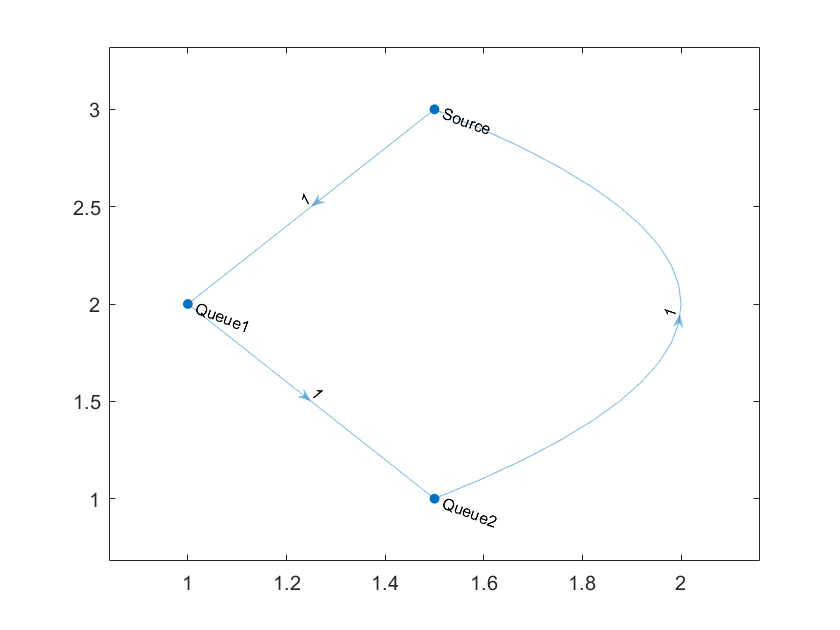
\includegraphics[width=7cm]{./images/getGraph_Stations.png}
  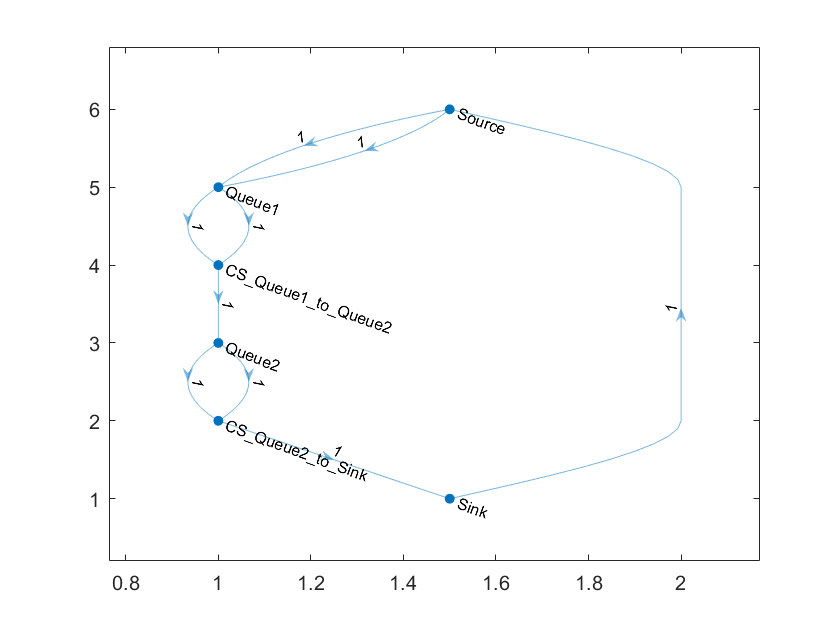
\includegraphics[width=7cm]{./images/getGraph_Nodes.png}
  \caption{\texttt{getGraph} function: station topology (left) and node topology (right) for a 2-class tandem queueing network with class-switching.}\label{FIG_getGraph}
\end{figure}

Furthermore, the graph properties concisely summarize the key features of the network
\begin{lstlisting}
>> G.Nodes
ans =
  2x5 table
      Name            Type           Sched    Jobs    ClosedClass1
    ________    _________________    _____    ____    ____________
    'Delay'     'Delay'       'inf'     5           1
    'Queue1'    'Queue'    'ps'      0           2
>> G.Edges
ans =
  3x4 table
          EndNodes          Weight    Rate        Class
    ____________________    ______    ____    ______________
    'Delay'     'Delay'      0.7        1     'ClosedClass1'
    'Delay'     'Queue1'     0.3        1     'ClosedClass1'
    'Queue1'    'Delay'        1      0.5     'ClosedClass1'
\end{lstlisting}
Here, \texttt{Edge.Weight} is the routing probability between the nodes, whereas \texttt{Edge.Rate} is the service rate of the source node.

\section{Model import and export}
%\section{Importing from BPMN}
%\section{Importing from JMT}
\textsc{Line} offers a number of scripts to import external models into \texttt{Network} object instances that can be analyzed through its solvers. %Similarly, a script is offered to convert a \texttt{Network} object instance into a MATLAB \texttt{.m} file for later re-use.
The available scripts are as follows:
\begin{itemize}
\item \texttt{JMT2LINE} imports a JMT simulation model (\texttt{.jsimg} or \texttt{.jsimw} file) instance.
\item \texttt{PMIF2LINE} imports a XML file containing a PMIF 1.0 model.
\end{itemize}
Both scripts require in input the filename and desired model name, and return a single output, e.g.,
\begin{lstlisting}
qn = PMIF2LINE([pwd,'\\examples\\data\\PMIF\\pmif_example_closed.xml'],'Mod1')
\end{lstlisting}
where \texttt{qn} is an instance of the \texttt{Network} class.

\texttt{Network} object can be saved in binary \texttt{.mat} files using MATLAB's standard \texttt{save} command. However, it is also possible to export a textual script that will dynamically recreate the same \texttt{Network} object. For example,
\begin{lstlisting}
example_closedModel_1; LINE2SCRIPT(model, 'script.m')
\end{lstlisting}
creates a new file \texttt{script.m} with code
\begin{lstlisting}
model = Network('model');
queue = Delay(model, 'Delay');
delay = Queue(model, 'Queue1', SchedStrategy.PS);
delay.setNumServers(1);
class1 = ClosedClass(model, 'ClosedClass1', 5, queue, 0);
queue.setService(class1, Cox2.fitMeanAndSCV(1.000000,1.000000));
delay.setService(class1, Cox2.fitMeanAndSCV(2.000000,1.000000));
P = cell(1);
P{1,1} = [0.7 0.3;1 0];
model.link(P);
\end{lstlisting}
that is equivalent to the model specified in \texttt{example\_closedModel\_1.m}.

\subsection{Creating a \textsc{Line} model using JMT}
Using the features presented in the previous section, one can create a model in JMT and automatically derive a corresponding \textsc{Line} script from it. For instance, the following command performs the import and translation into a script, e.g.,
\begin{lstlisting}
LINE2SCRIPT(JMT2LINE('myModel.jsimg'),'myModel.m')
\end{lstlisting}
transforms and save the given JSIMgraph model into a corresponding \textsc{Line} model.

\textsc{Line} also gives two static functions to inspect \texttt{jsimg} and \texttt{jsimw} files before conversion, i.e.,
\texttt{SolverJMT.jsimgOpen} and \texttt{SolverJMT.jsimwOpen} require as an input parameter only the JMT file name, e.g., 'myModel.jsimg'.

